\subsection{Track selection}
The track selection for 5.02 TeV Pb+Pb follows the standard cut implemented in the $\verb|xAOD ToolInDet|$:

Loose quality cut is denoted as $\verb|HILoose|$ and is defined as:
\begin{itemize}
\item $p_{\text{T}}>500$ MeV;
\item number of Pixel hits $>0$;
\item number of SCT hits + dead sensors $\geq 6$;
\item if IBL hit is expected: at least 1 IBL hit required;
\item if no IBL hit is expected: a Layer-0 hit if expected;
\item $|d_0|\leq 1.5$ mm;
\item $|z_0-z_{\text{vtx}}|*\text{sin}\theta\leq 1.5$ mm;
\end{itemize}
where "ndf" denotes number of degree of freedom of the track.

Tight quality cut is denoted as $\verb|HITight|$ and is defined as:
\begin{itemize}
\item $p_{\text{T}}>500$ MeV;
\item *** number of Pixel hits $>1$;
\item *** number of SCT hits + dead sensors $\geq 8$;
\item if IBL hit is expected: at least 1 IBL hit required;
\item if no IBL hit is expected: a Layer-0 hit if expected;
\item *** $|d_0|\leq 1.0$ mm;
\item *** $|z_0-z_{\text{vtx}}|*\text{sin}\theta\leq 1.0$ mm;
\item *** $\chi^2/\text{ndf}\leq 6$;
\end{itemize}
where the differences compared with loose cut are highlighted with "***". In this analysis, the default track selection is the loose quality cut, and tight quality cut is used as a systematic check and is discussed in Section.~\ref{sec:sys}. We prefer $\verb|HILOOSE|$ over $\verb|HITIGHT|$ mainly because there are more particles remaining with the loose cut, which results in smaller statistical uncertainties. The loose and tight cuts are determined by evaluating the tracking efficiency and fake rates in the Monte-Carlo samples with same detector conditions as during the data taking and these two cuts results in relatively lower fake rates with high tracking efficiency.



\subsection{Tracking in Monte-Carlo}
To estimate the tracking efficiency and fake rate in 5.02 TeV Pb+Pb, HIJING Monte-Carlo samples with similar detector conditions and flow after-burner~\cite{Poskanzer:1998yz} are used:
\begin{itemize}
\item \verb|mc15_5TeV.420000.Hijing_PbPb_5p02TeV_MinBias_Flow_JJFV6.recon.AOD.| \\
\verb|e4962_a868_s2921_r9447|
\end{itemize}

Within the reconstructed tracks, the primary tracks $N_{ch}^{primary}$ are defined as:
\begin{itemize}
\item pass the loose track quality selection;
\item truth match probability $> 0.5$;
\item associated truth particle is a primary particle;
\end{itemize}
where primary particle is defined on the truth level:
\begin{itemize}
\item status $= 1$, charge $!= 0$;
\item $p_{\text{T}}>200$ MeV;
\item $|\eta|\leq 2.5$;
\item $0 < \text{Barcode} < 2\text{E}5$;
\item strange baryons are excluded;
\end{itemize}

The tracking efficiency $\epsilon$ is then defined as:
\begin{equation}
\epsilon(p_{\text{T}},\eta,\text{centrality})\equiv \frac{N_{ch}^{primary}}{N_{ch}^{truth}}
\end{equation}
where $N_{ch}^{primary}$ denotes the number of primary tracks on reconstructed level and $N_{ch}^{truth}$ denotes the number of primary particles on the truth level, all of which passed the loose quality selection.

The fake track is defined as:
\begin{itemize}
\item pass the loose track quality selection;
\item fulfill one of the following:
\begin{itemize}
\item truth match probability $< 0.5$;
\item not associated with truth particles;
\item Barcode $= 0$ of associated truth particle;
\end{itemize}
\end{itemize}

The fraction of fake tracks $f$ is defined as:
\begin{equation}
f(p_{\text{T}},\eta,\text{centrality})\equiv \frac{N_{ch}^{fake}}{N_{ch}^{primary}+N_{ch}^{fake}}
\end{equation}
where $N_{ch}^{fake}$ denotes the number of fake tracks.

To compensate the contribution from fake tracks, the efficiency $\epsilon$ can be corrected by defining $\epsilon^{'}$:
\begin{equation}
\epsilon^{'}(p_{\text{T}},\eta,\text{centrality})\equiv \frac{N_{ch}^{primary}+N_{ch}^{fake}}{N_{ch}^{truth}}=\frac{\epsilon}{1-f}
\end{equation}
where an additional correction of fake rates $1-f$ is added to the tracking efficiency $\epsilon$.



\subsection{Efficiency}
The tracking efficiency map used in this analysis is borrowed from Run 2 $v_n$ analysis~\cite{Burka:2151932}, which is evaluated as a function of $p_{\text{T}}, \eta$ and centrality. To estimate the tracking efficiency, the track selection follows the loose quality cut. The tracking efficiency $\epsilon(\eta)$ are shown in Fig.~\ref{fig:PbPb502_trkEff}, for different $p_{\text{T}}$ ranges and centrality. $\epsilon(\eta)$ is highest in mid-rapidity $-1<\eta<1$, and decreases by $~20\%$ in forward-rapidity. As collision moves to peripheral, the efficiency increases. The tracking efficiency slightly increases towards higher $p_{\text{T}}$. Efficiency from $\verb|HILOOSE|$ is higher than $\verb|HITIGHT|$ as expected.
\begin{figure} [H]
\centering
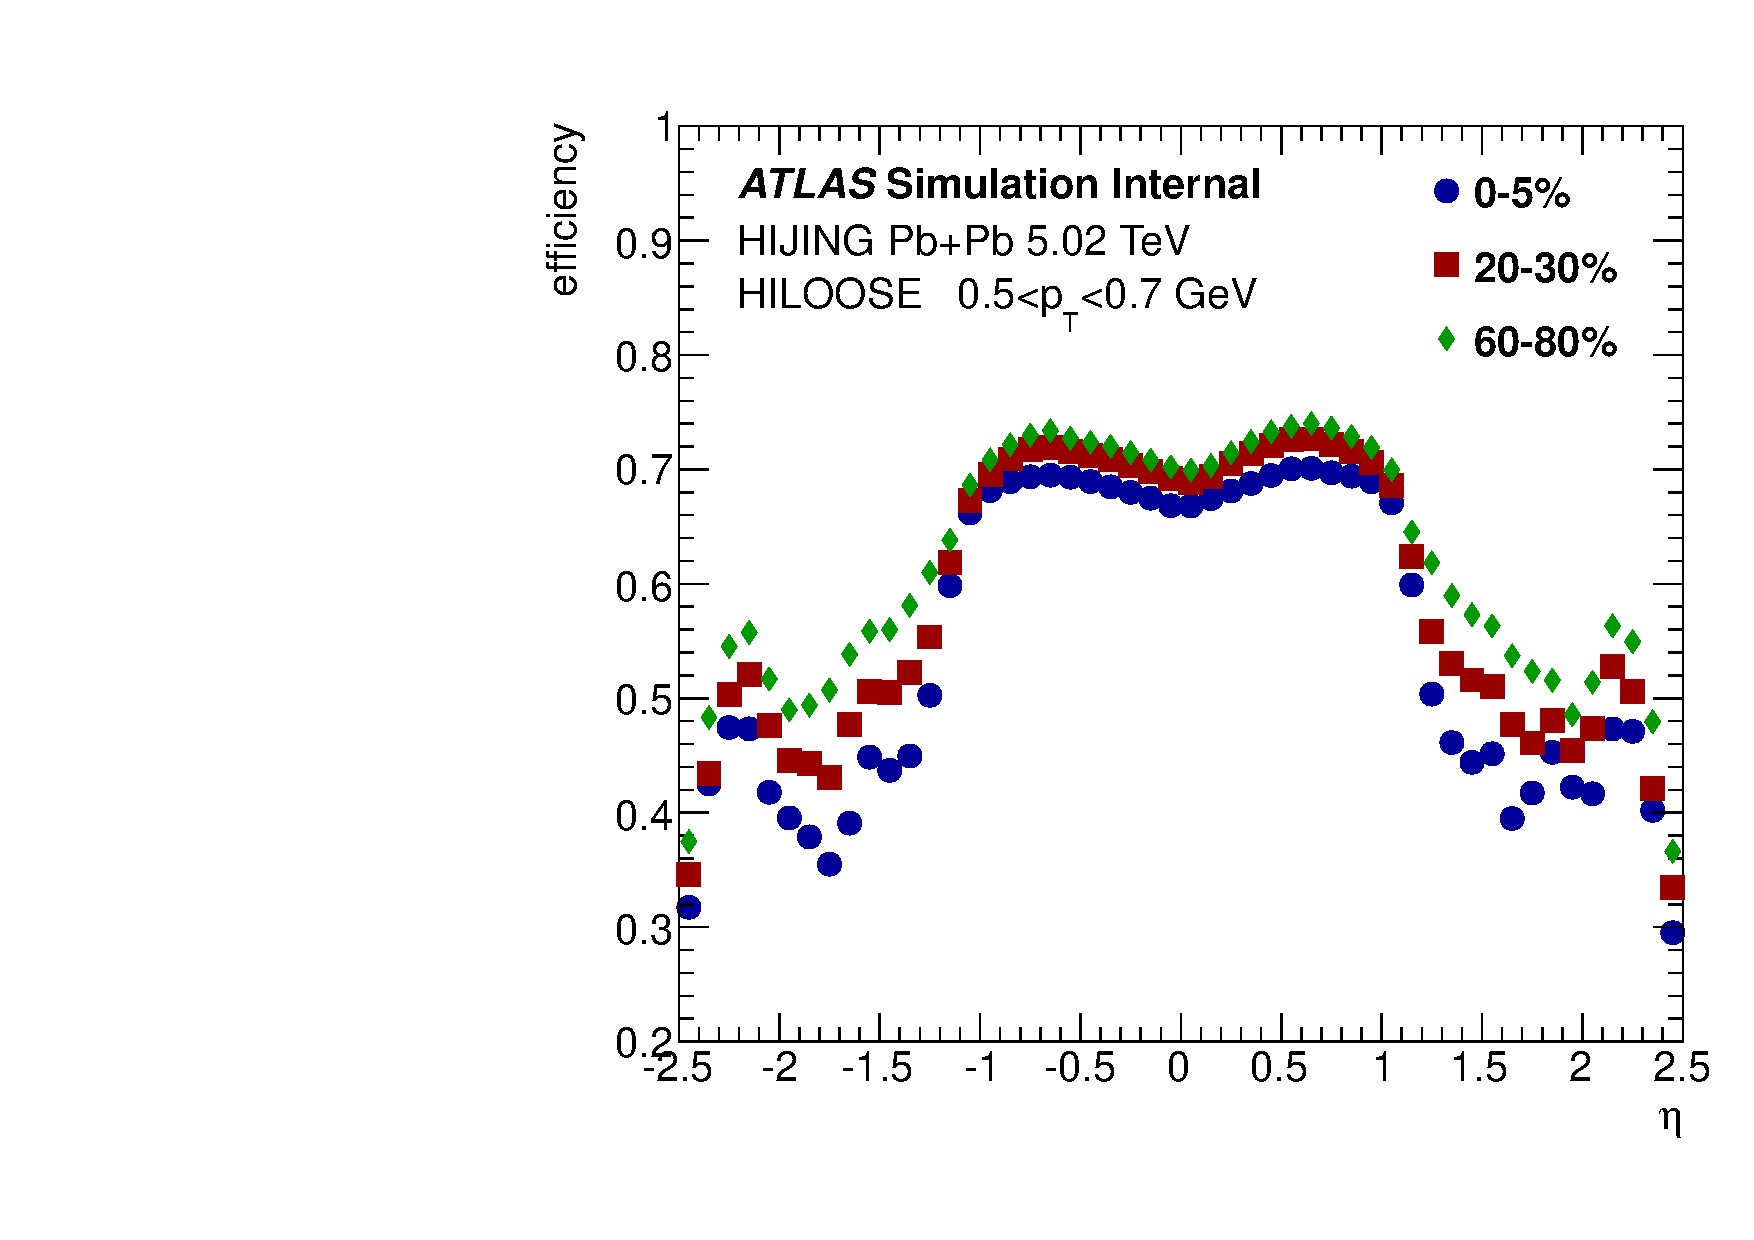
\includegraphics[width=.32\linewidth]{figs/sec_trkSel/PbPb502/PbPb502_LOOSE_eff_Pt0.pdf}
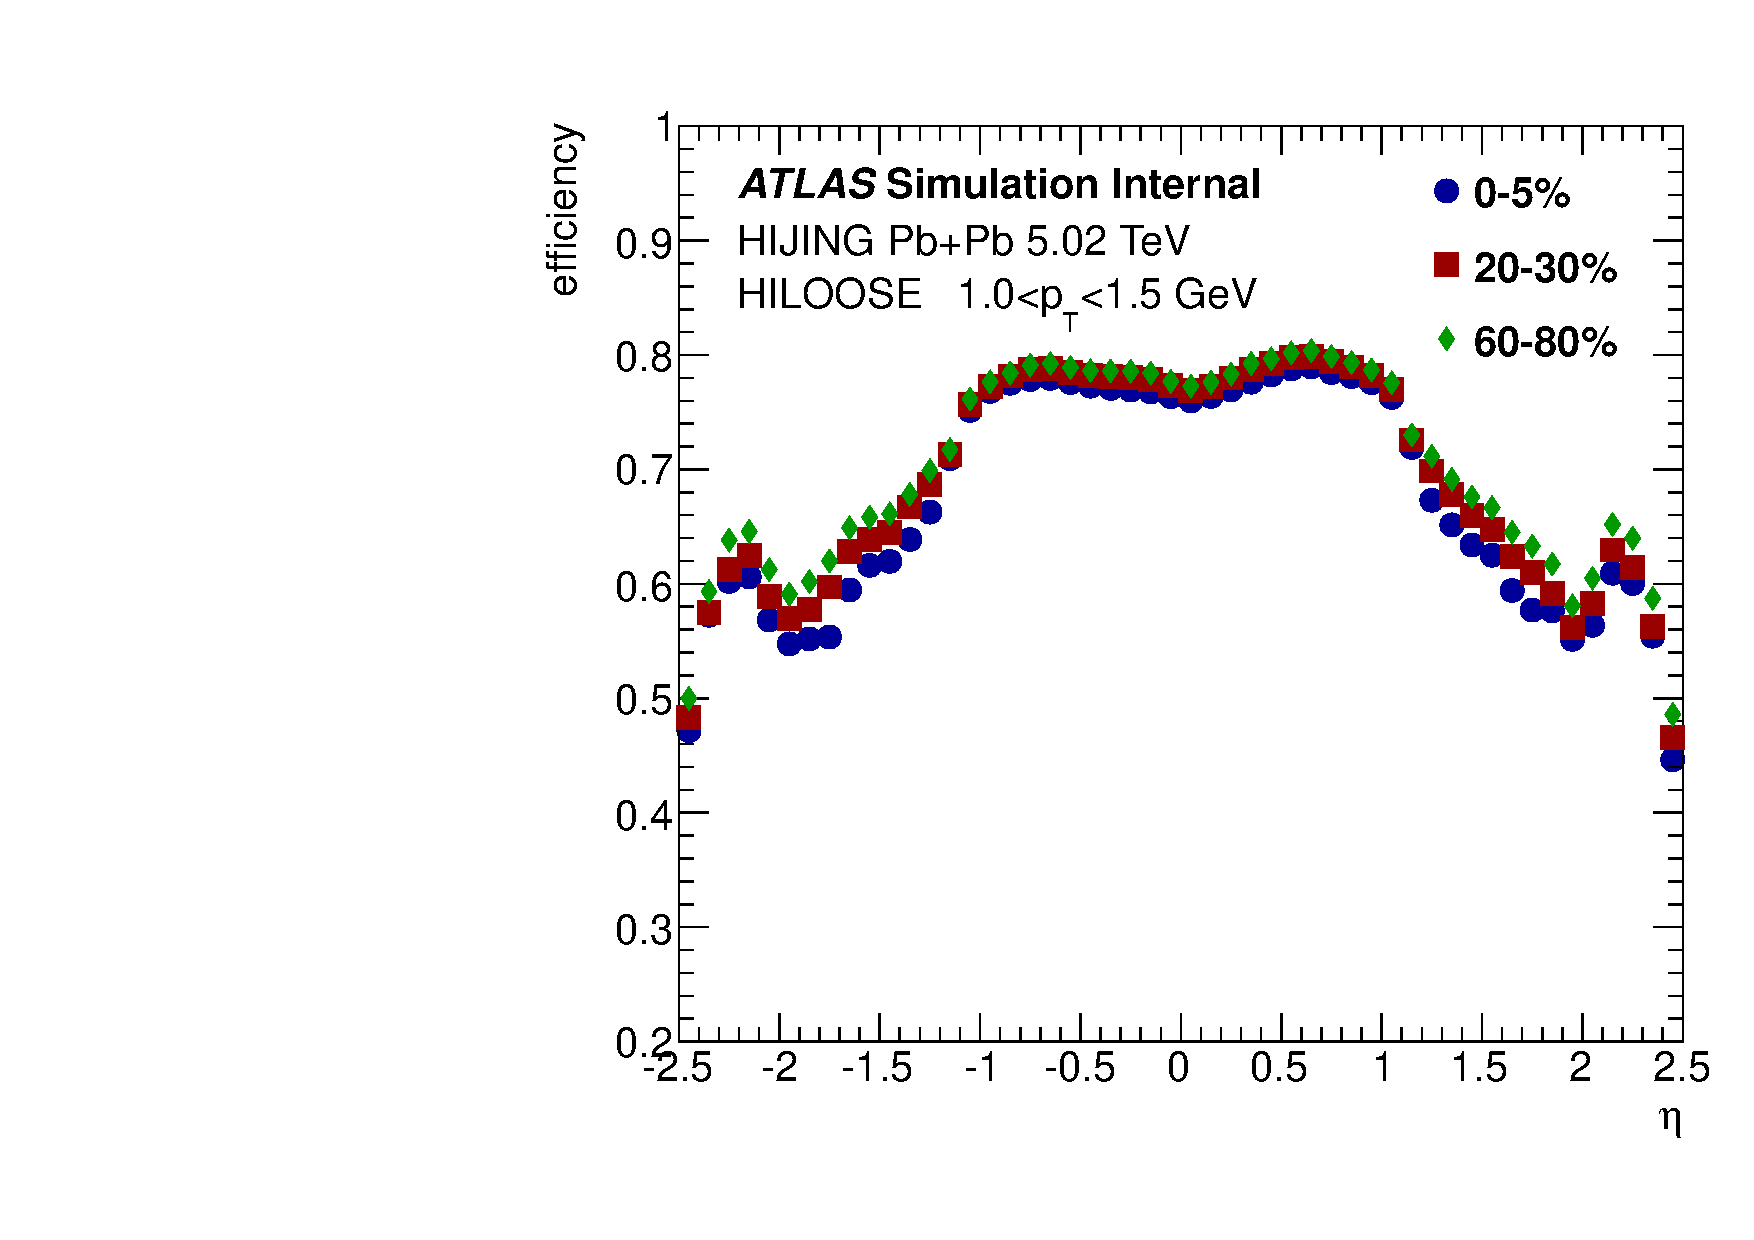
\includegraphics[width=.32\linewidth]{figs/sec_trkSel/PbPb502/PbPb502_LOOSE_eff_Pt2.pdf}
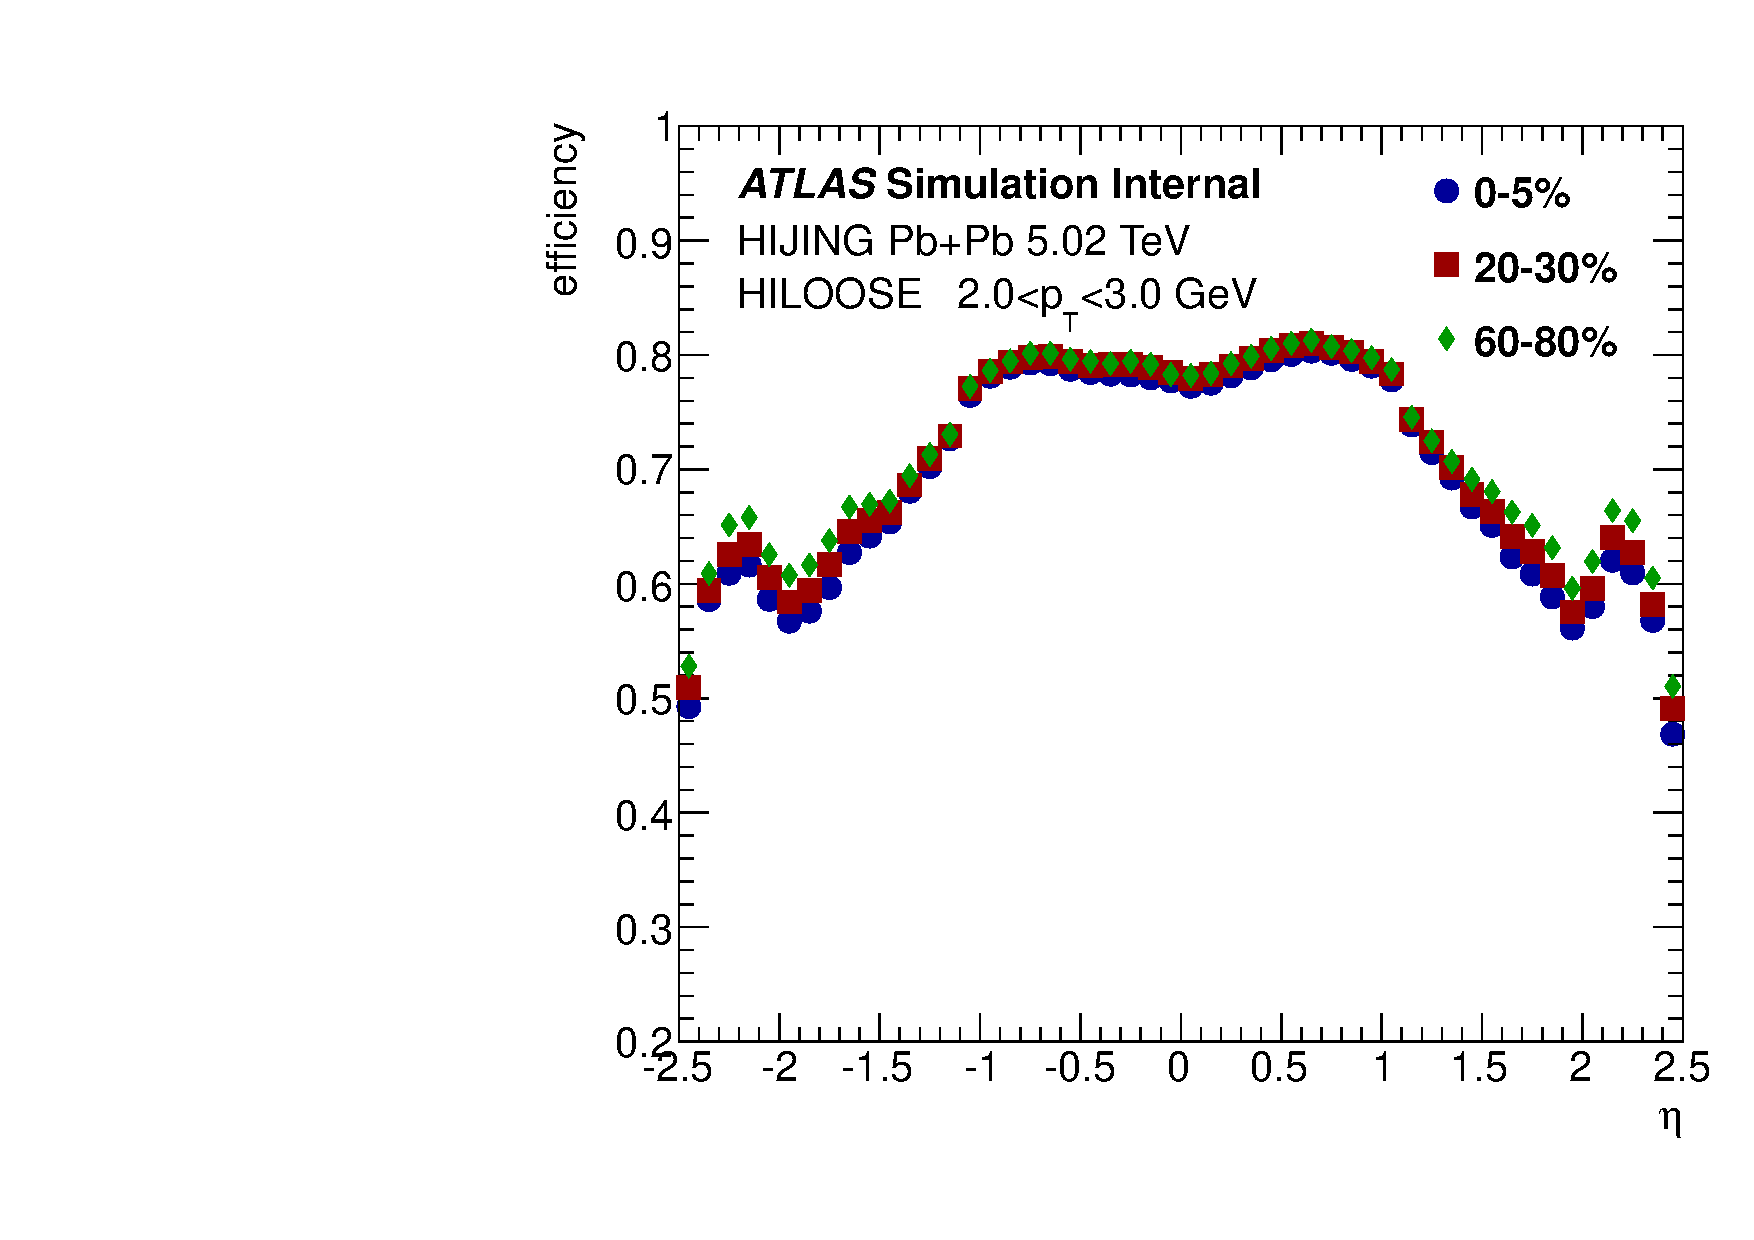
\includegraphics[width=.32\linewidth]{figs/sec_trkSel/PbPb502/PbPb502_LOOSE_eff_Pt4.pdf}
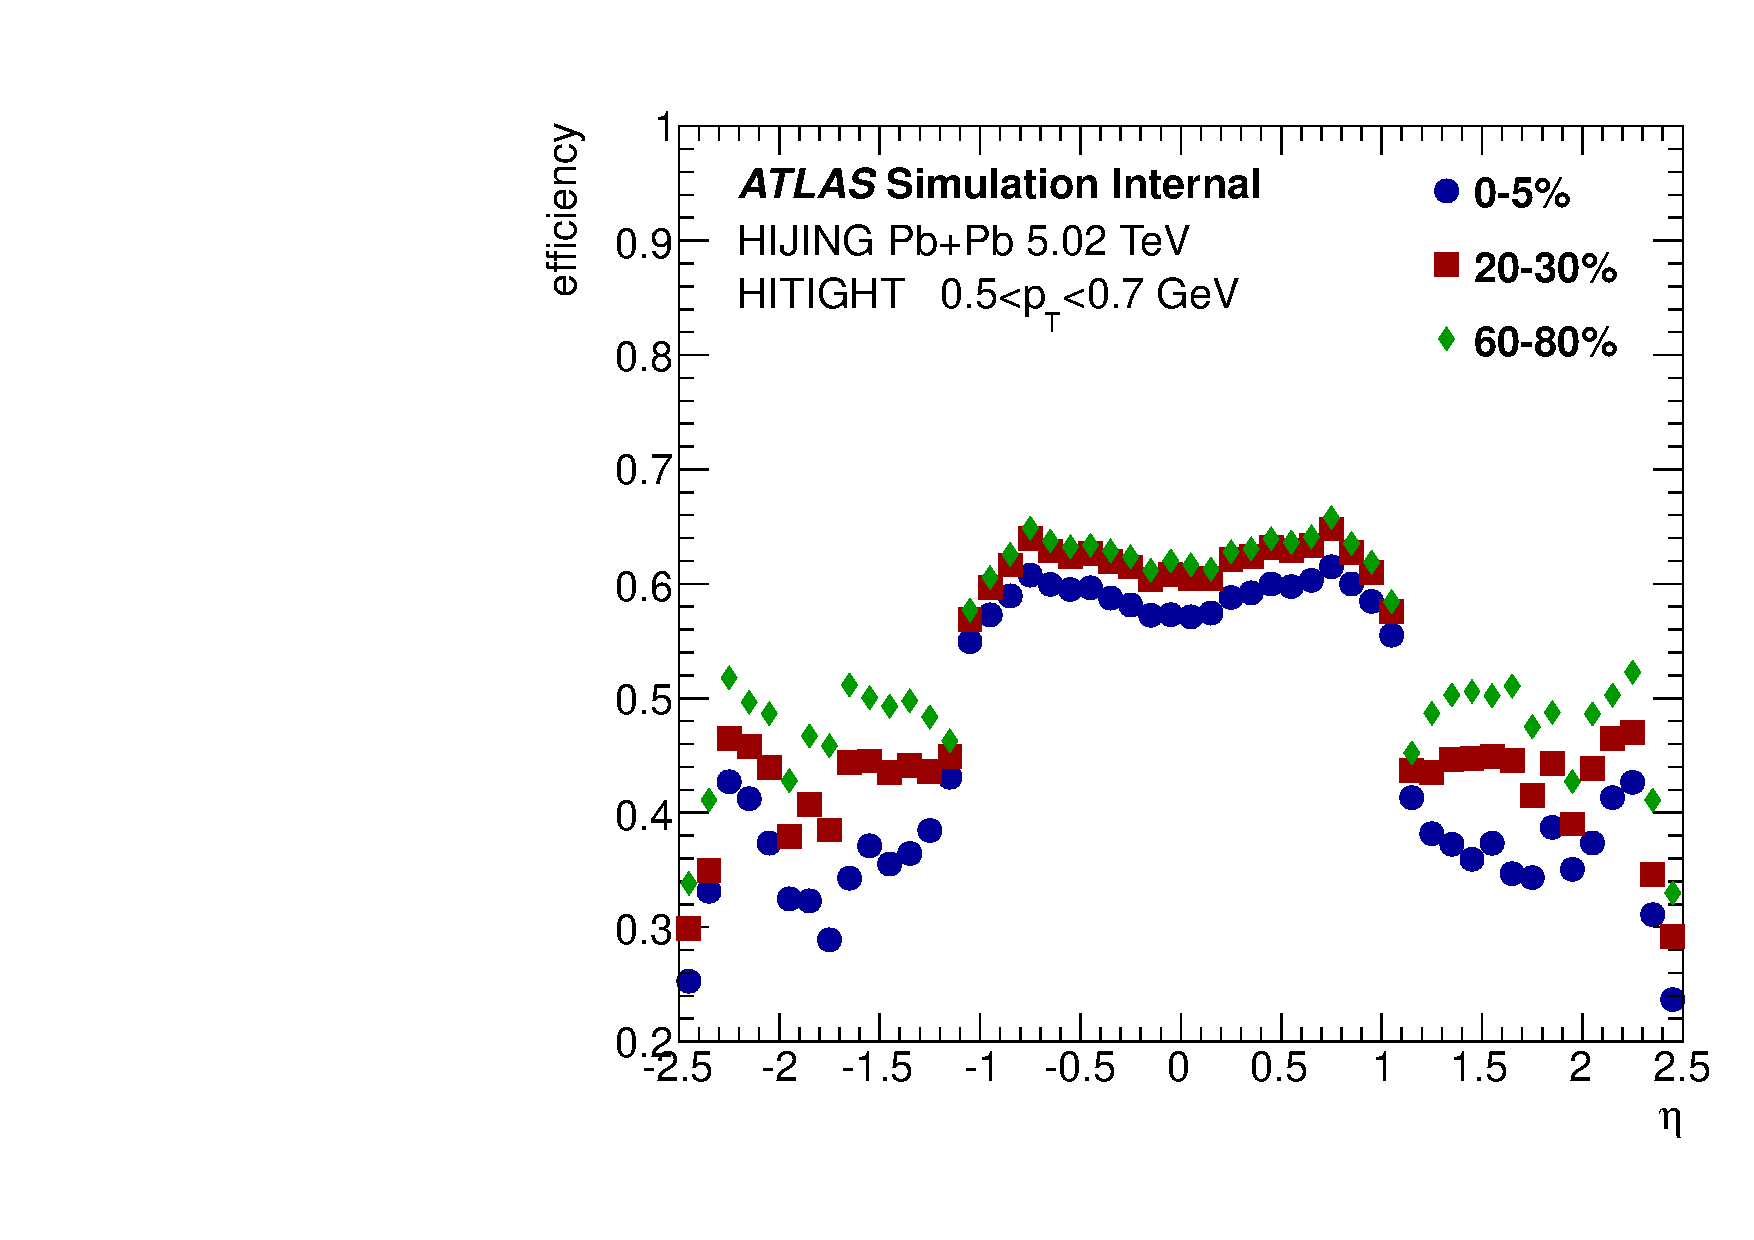
\includegraphics[width=.32\linewidth]{figs/sec_trkSel/PbPb502/PbPb502_TIGHT_eff_Pt0.pdf}
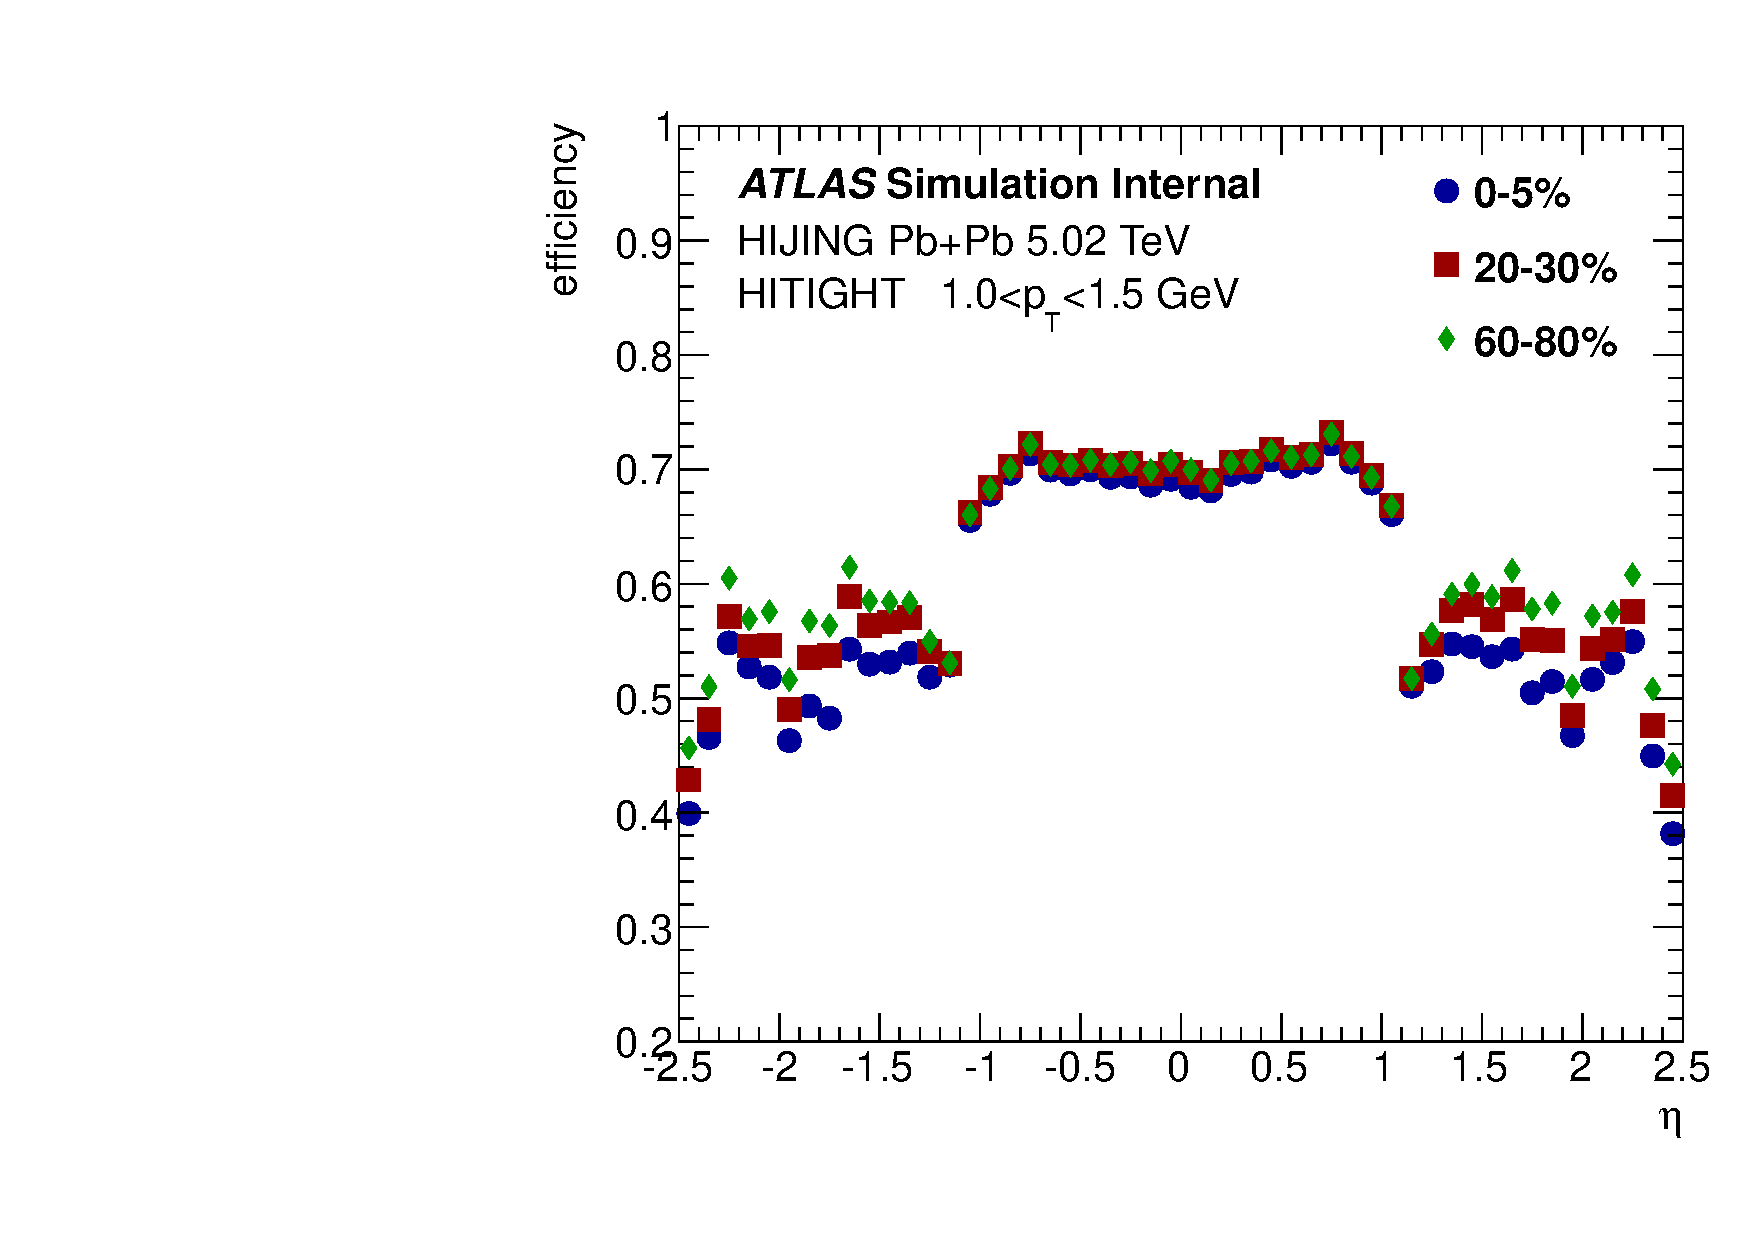
\includegraphics[width=.32\linewidth]{figs/sec_trkSel/PbPb502/PbPb502_TIGHT_eff_Pt2.pdf}
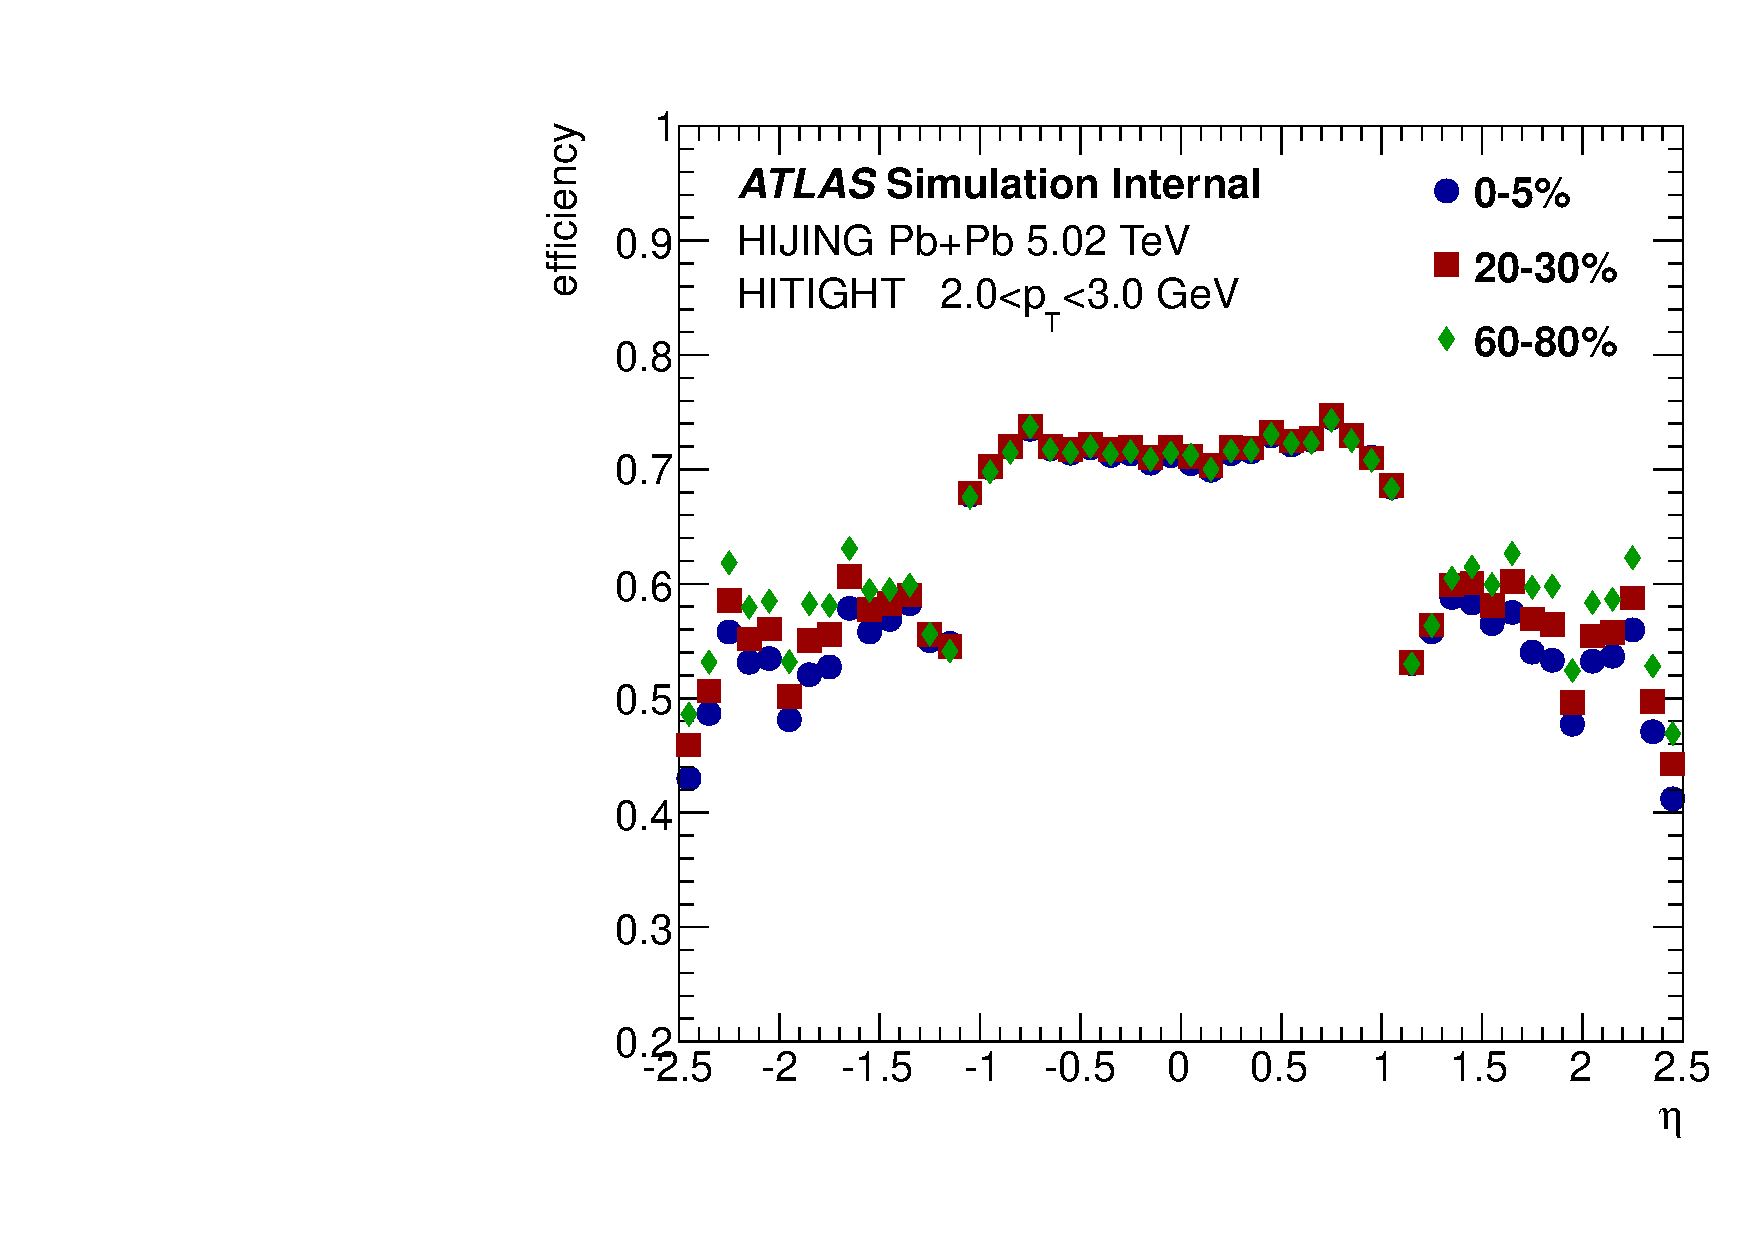
\includegraphics[width=.32\linewidth]{figs/sec_trkSel/PbPb502/PbPb502_TIGHT_eff_Pt4.pdf}
\caption{5.02 TeV Pb+Pb tracking efficiency $\epsilon(\eta)$, for different $p_{\text{T}}$ ranges and centralities. Top row is for loose track quality cut (default) and bottom row is for tight cut.}
\label{fig:PbPb502_trkEff}
\end{figure}



\subsection{Fakes}
Since one of the focuses in this analysis is on ultra-central collisions, fake rate correction $1-f$ were applied to the efficiency $\epsilon$ and each track is weighted by $(1-f)/\ \epsilon$. The fake rates map is also borrowed from Run 2 $v_n$ analysis~\cite{Burka:2151932}, which is evaluated as a function of $p_{\text{T}}, \eta$ and centrality. To estimate the fraction of fake tracks, the track selection follows the loose quality cut. The fake rate $f(\eta)$ are shown in Fig.~\ref{fig:PbPb502_trkFak}, for different $p_{\text{T}}$ ranges and centrality. $f(\eta)$ is lowest in mid-rapidity $-1<\eta<1$, and increases by more than 2 times in forward-rapidity. As collision moves to peripheral, the fake rate significantly decreases. The fake rate decreases significantly towards higher $p_{\text{T}}$. Fake rate from $\verb|HILOOSE|$ is higher than $\verb|HITIGHT|$ as expected.
\begin{figure} [H]
\centering
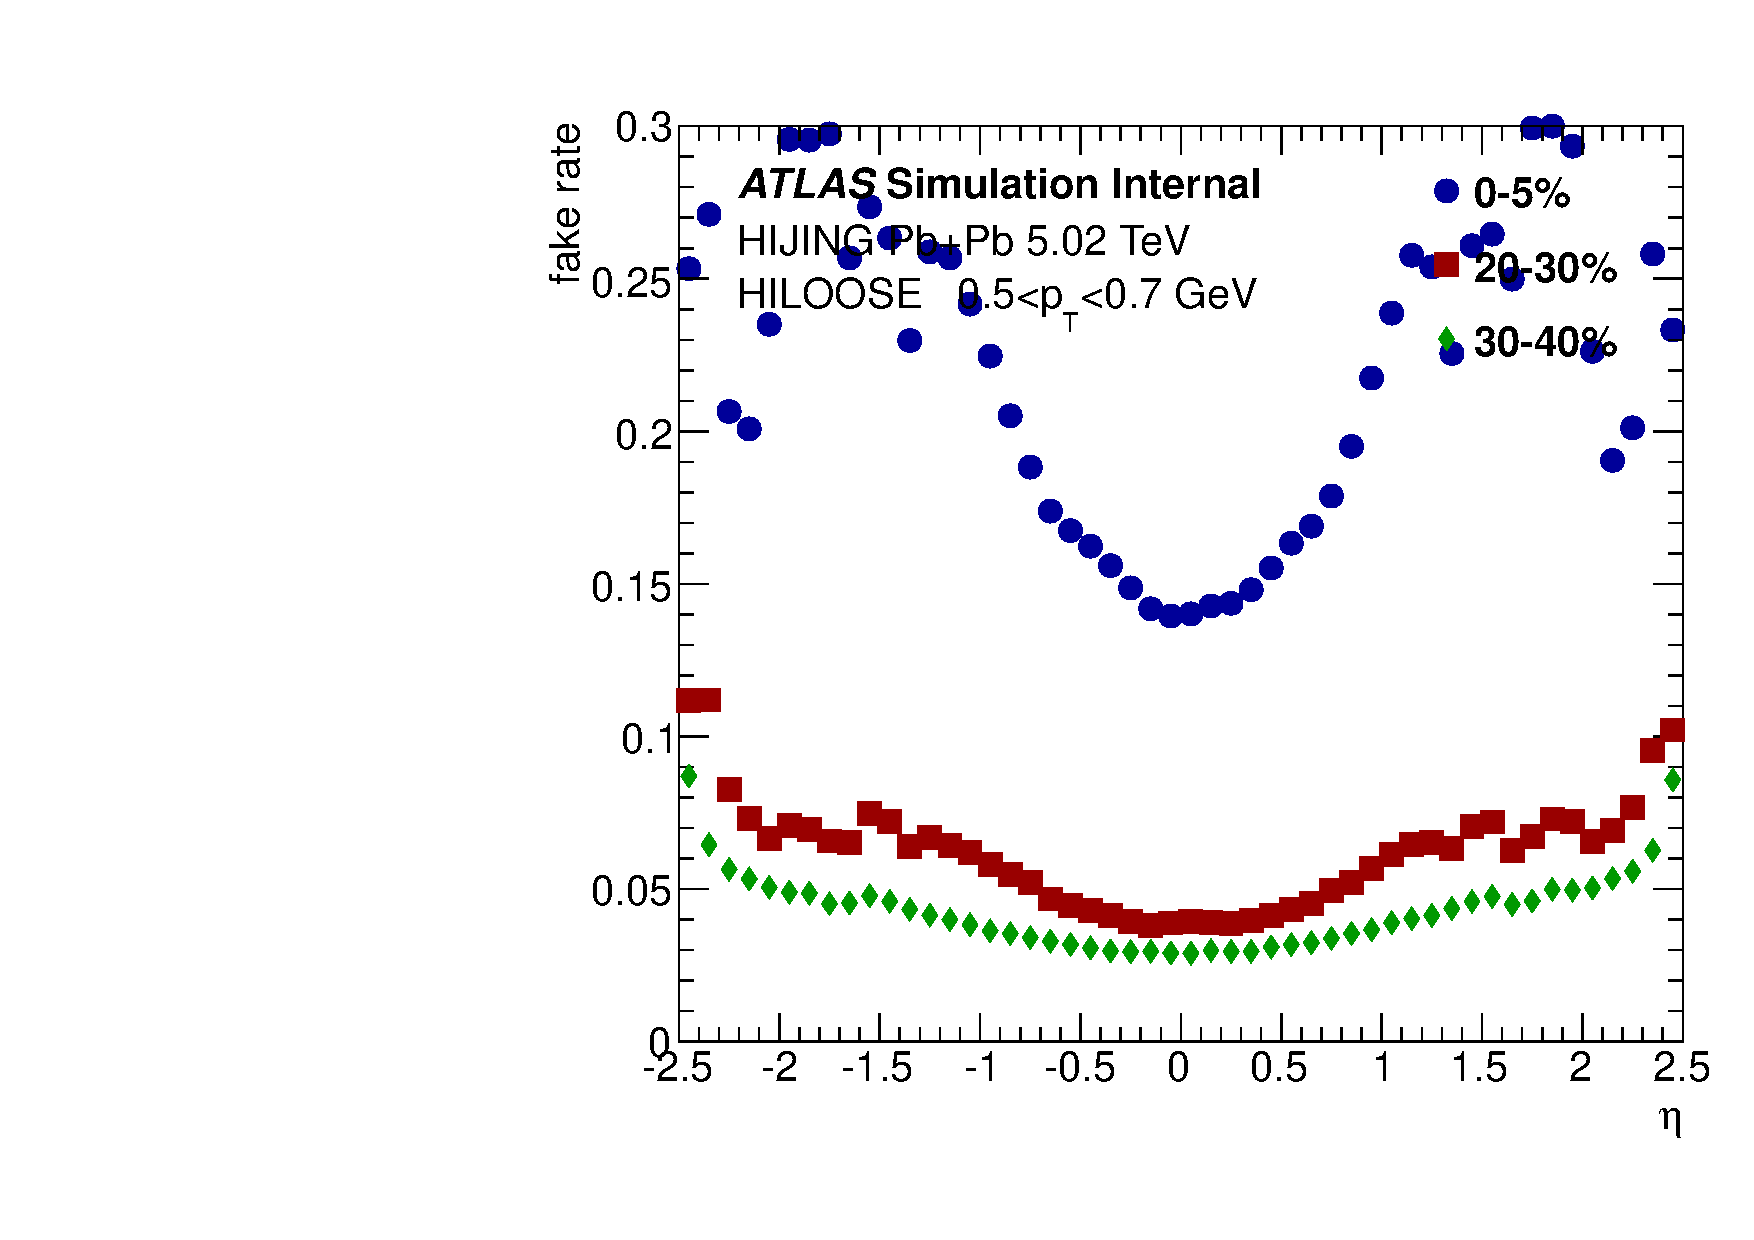
\includegraphics[width=.32\linewidth]{figs/sec_trkSel/PbPb502/PbPb502_LOOSE_fak_Pt0.pdf}
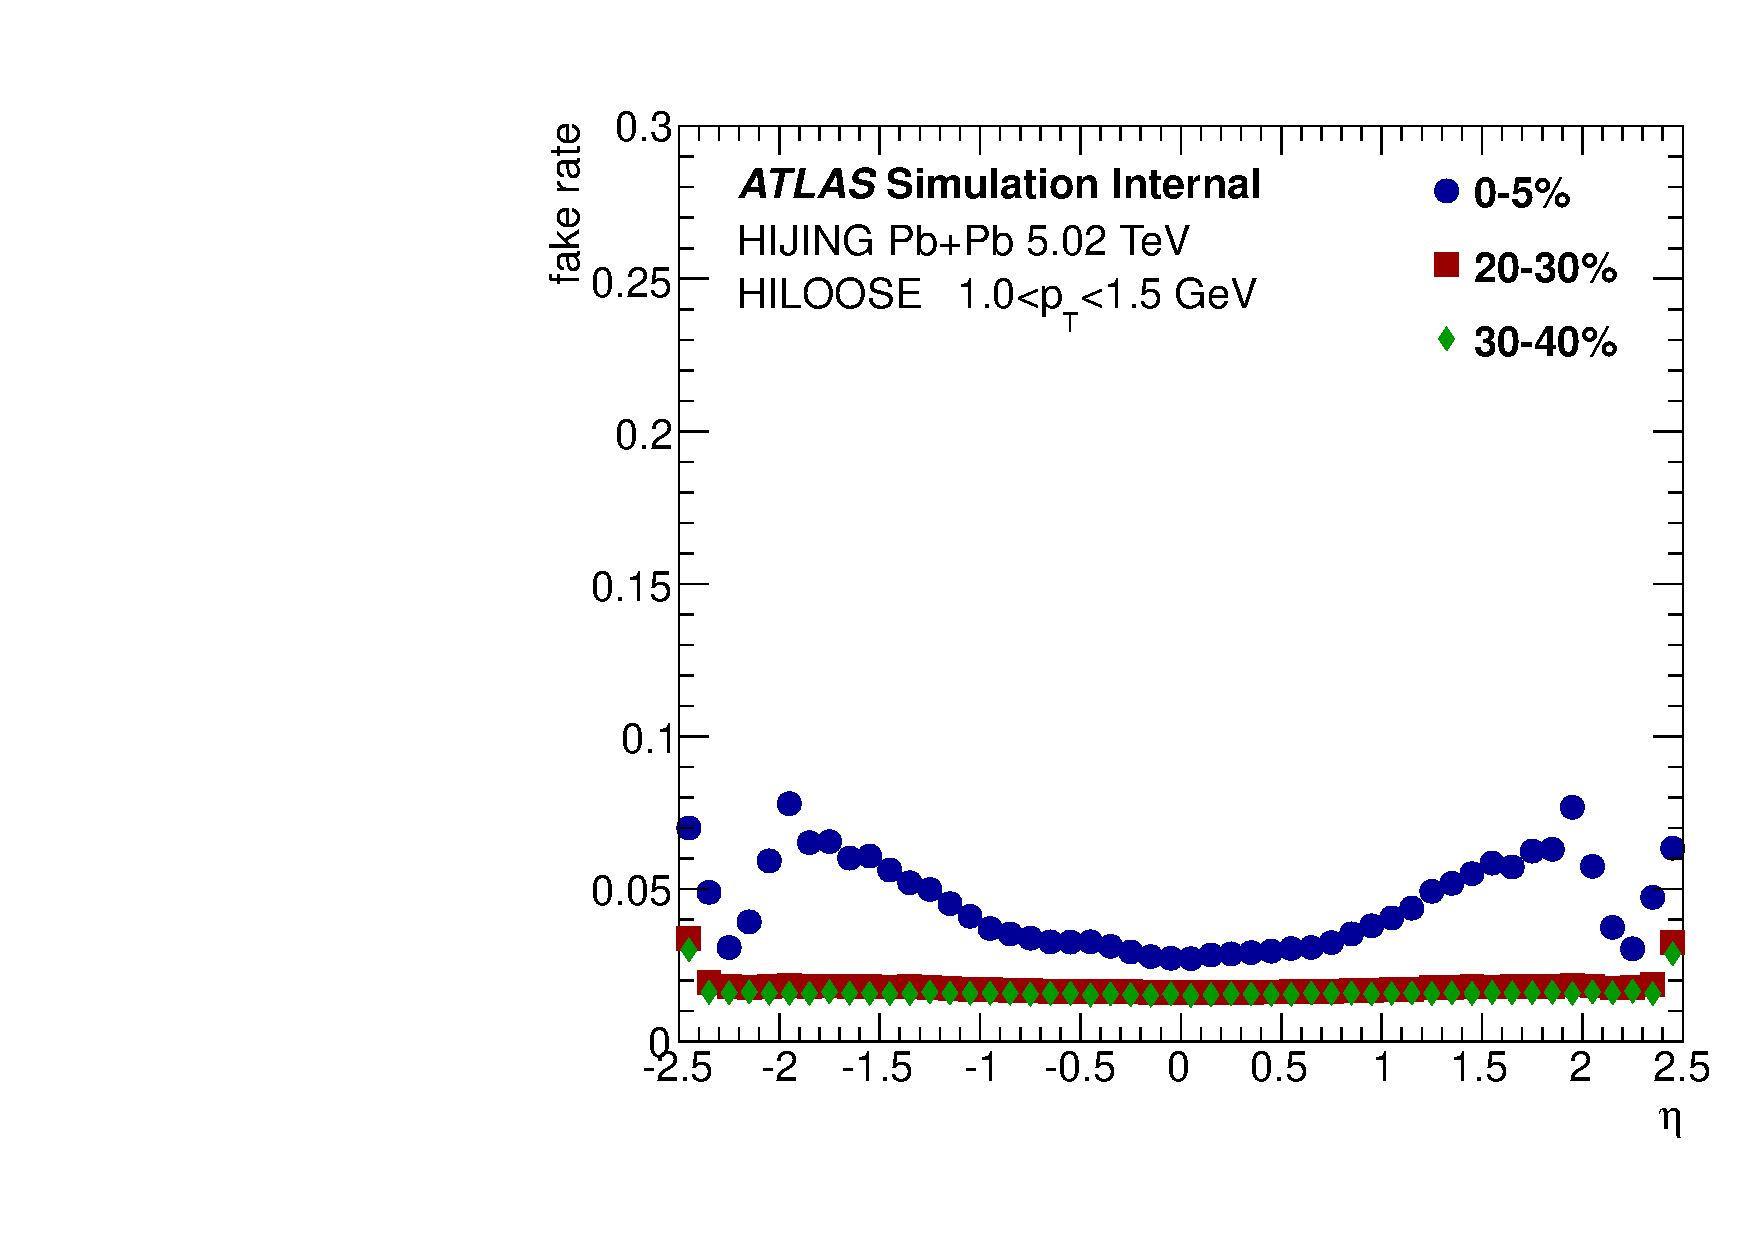
\includegraphics[width=.32\linewidth]{figs/sec_trkSel/PbPb502/PbPb502_LOOSE_fak_Pt2.pdf}
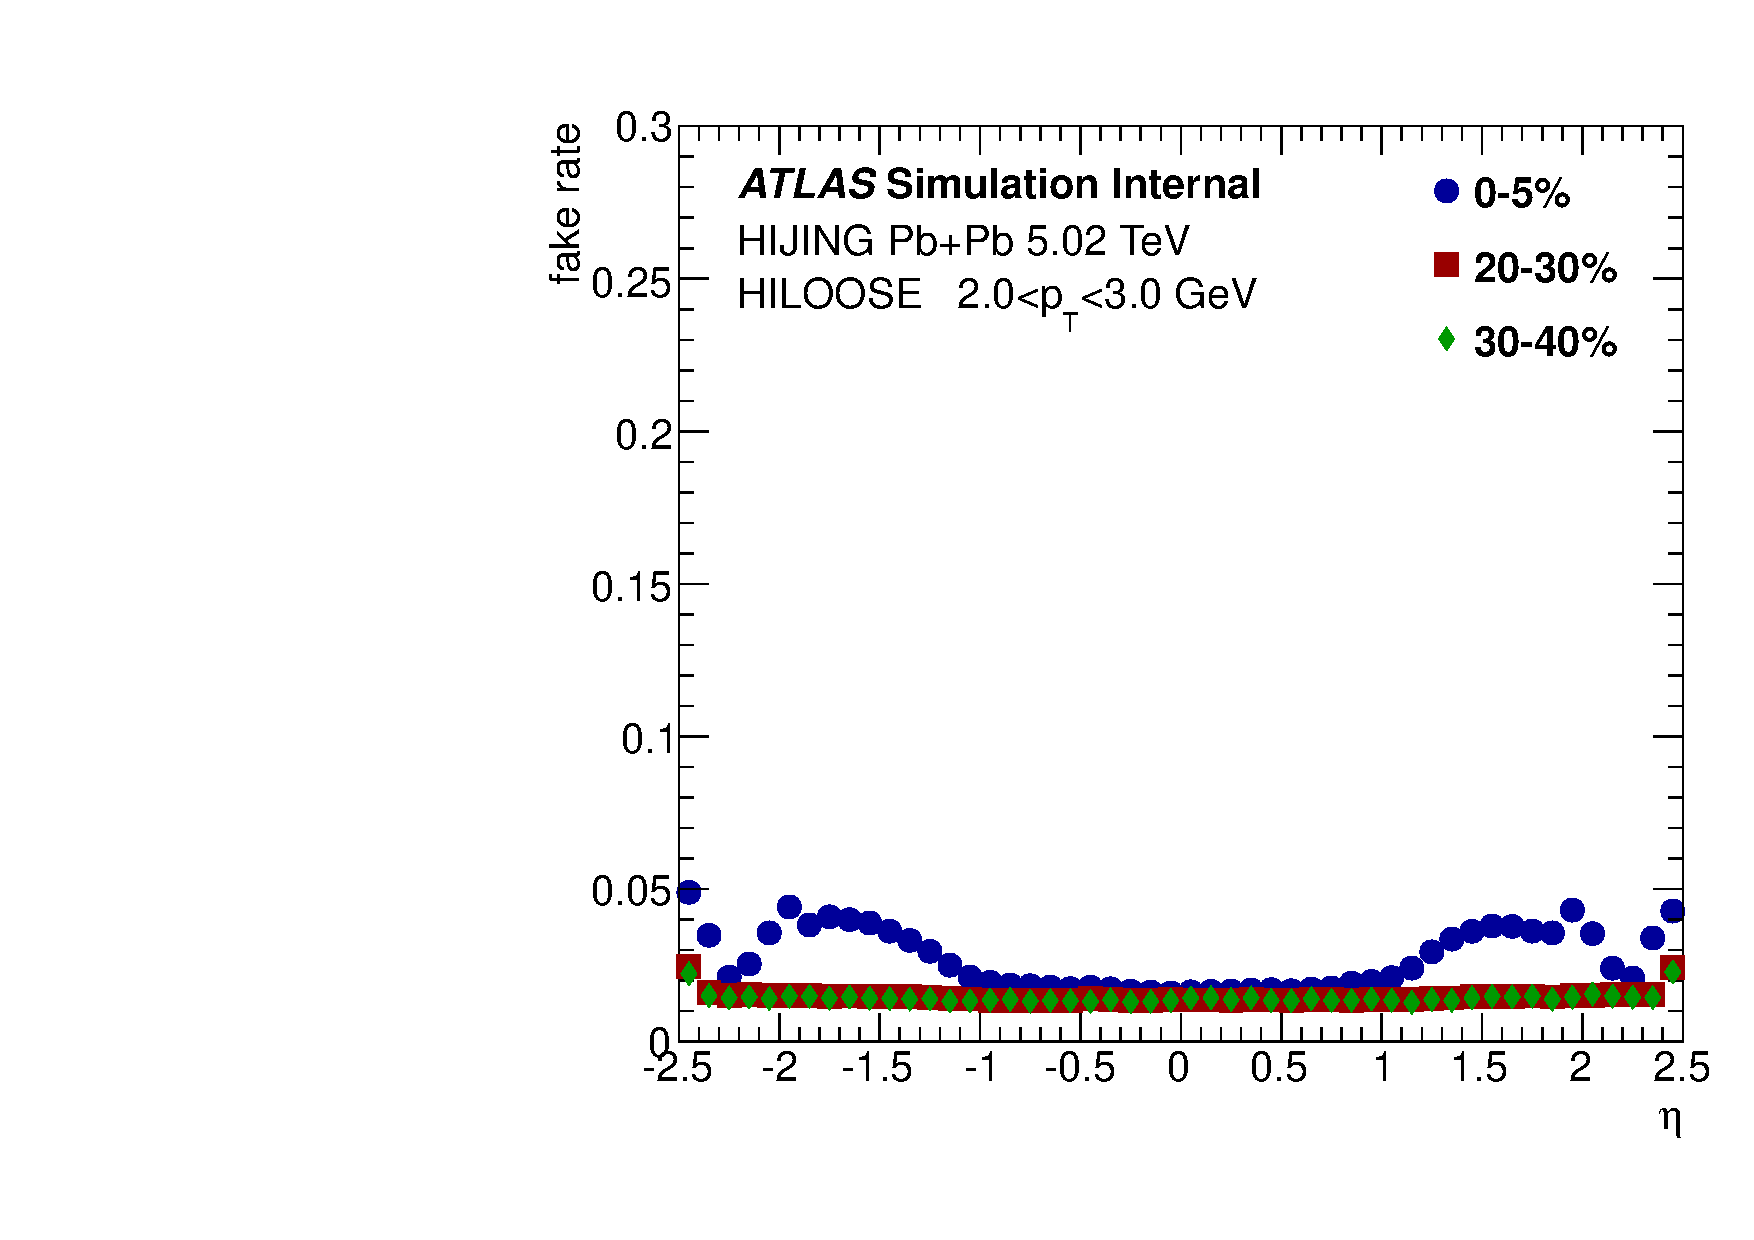
\includegraphics[width=.32\linewidth]{figs/sec_trkSel/PbPb502/PbPb502_LOOSE_fak_Pt4.pdf}
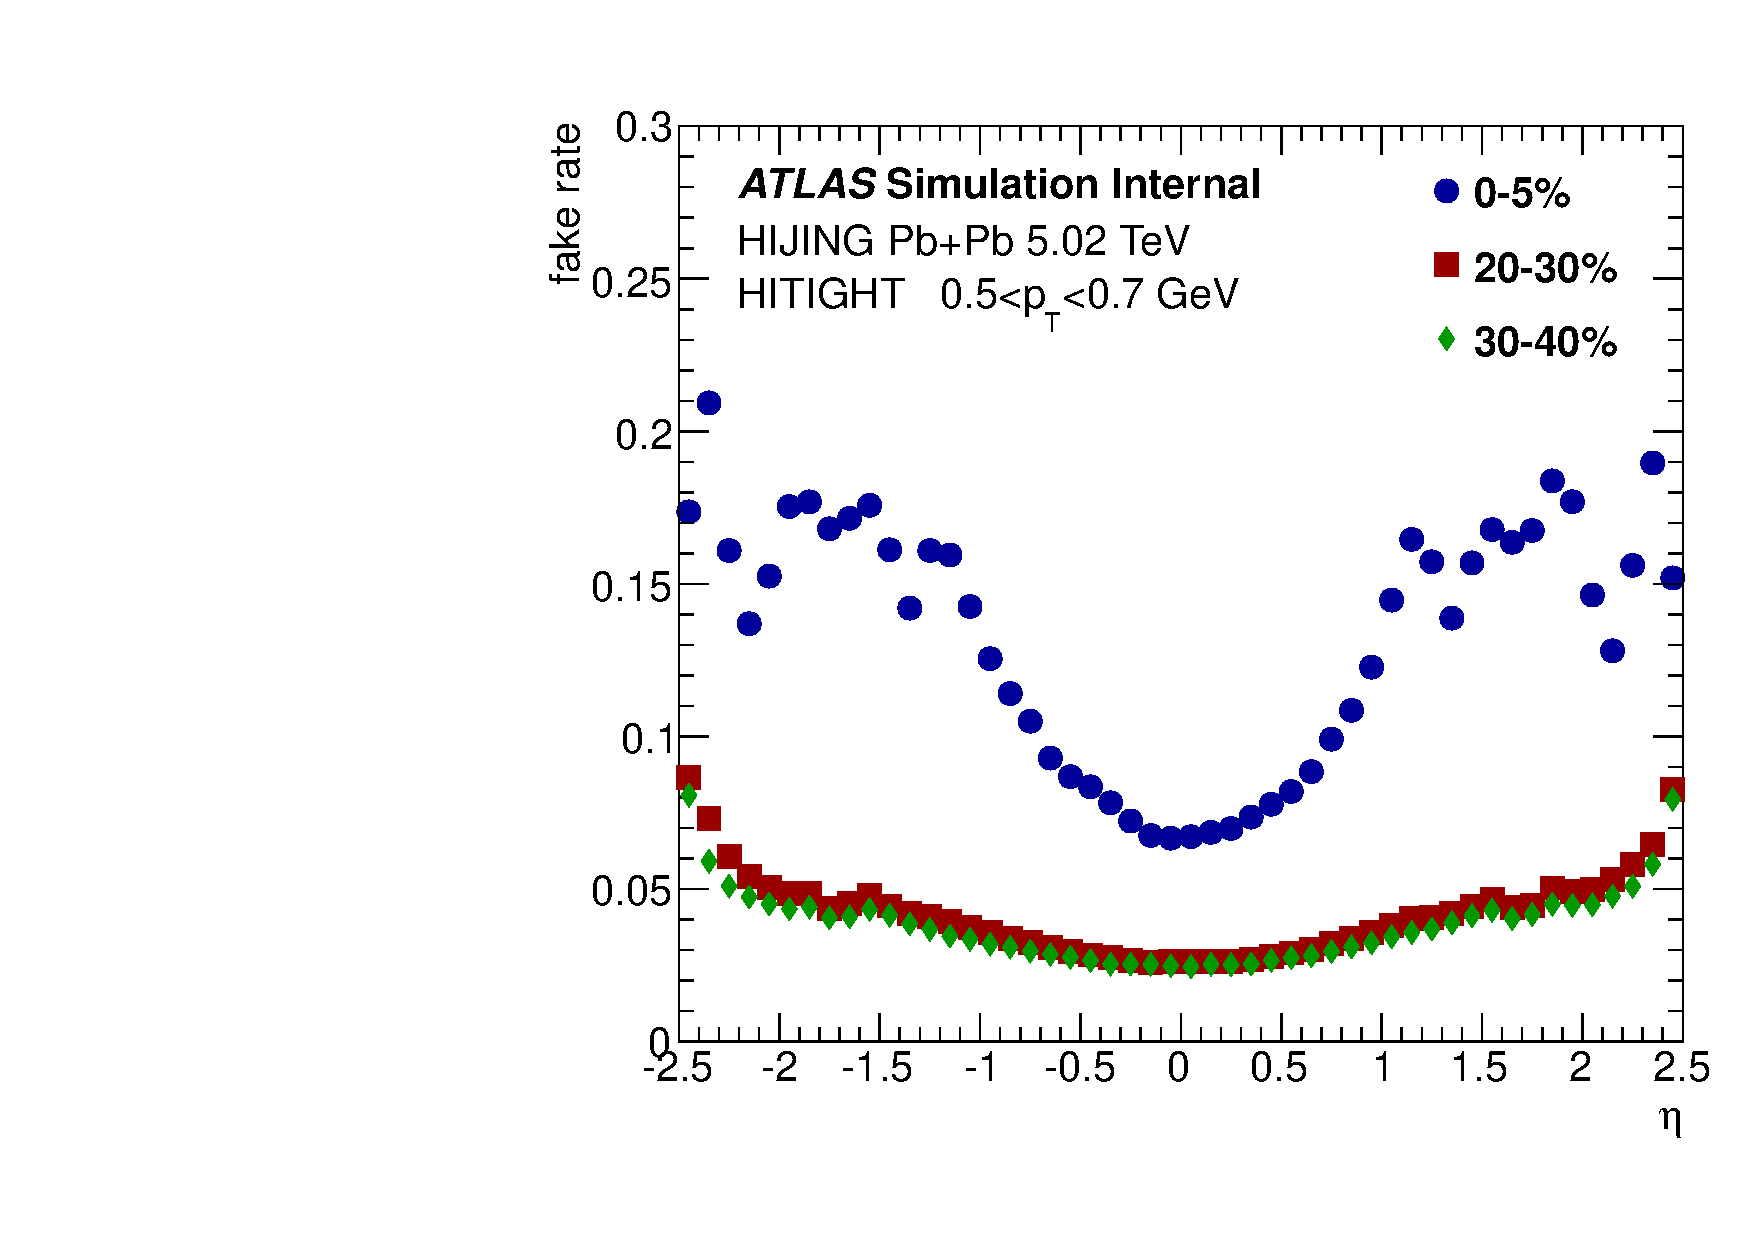
\includegraphics[width=.32\linewidth]{figs/sec_trkSel/PbPb502/PbPb502_TIGHT_fak_Pt0.pdf}
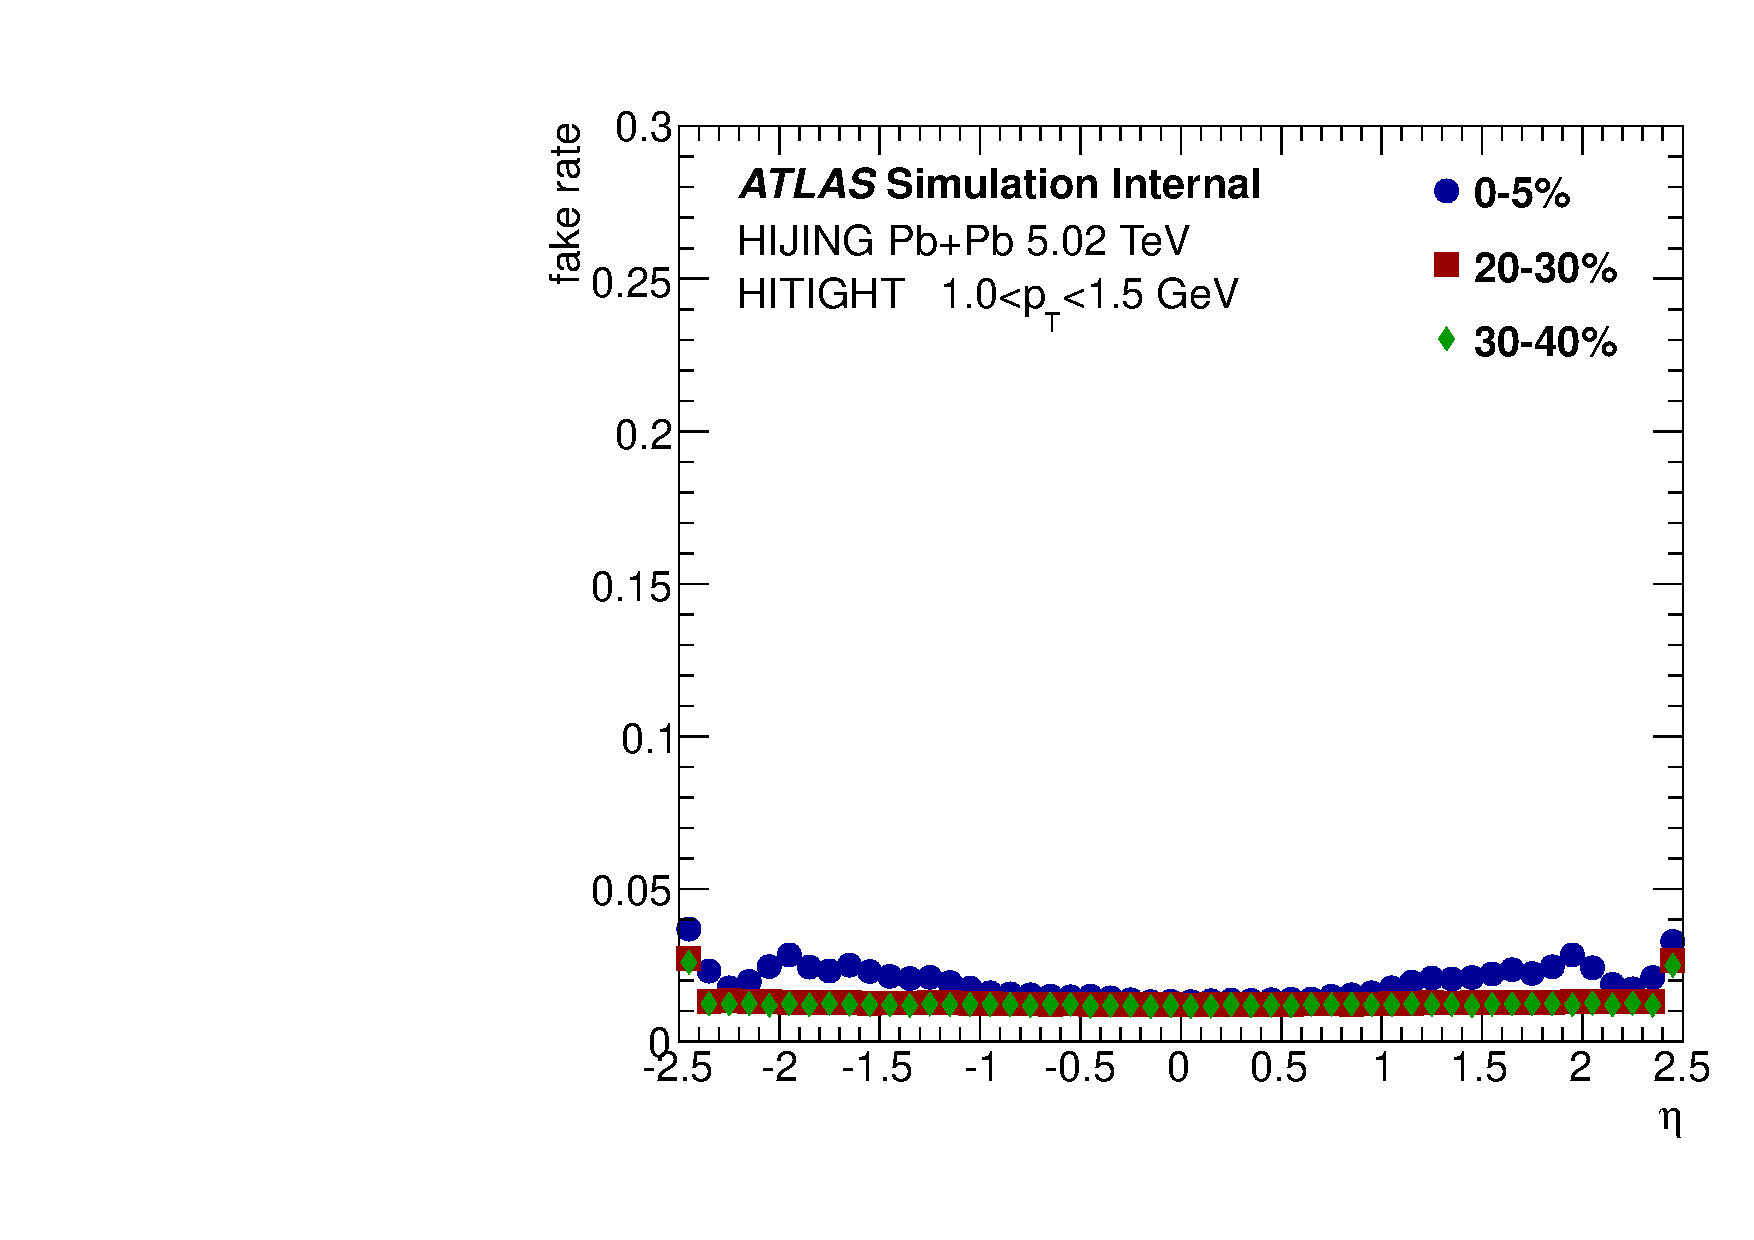
\includegraphics[width=.32\linewidth]{figs/sec_trkSel/PbPb502/PbPb502_TIGHT_fak_Pt2.pdf}
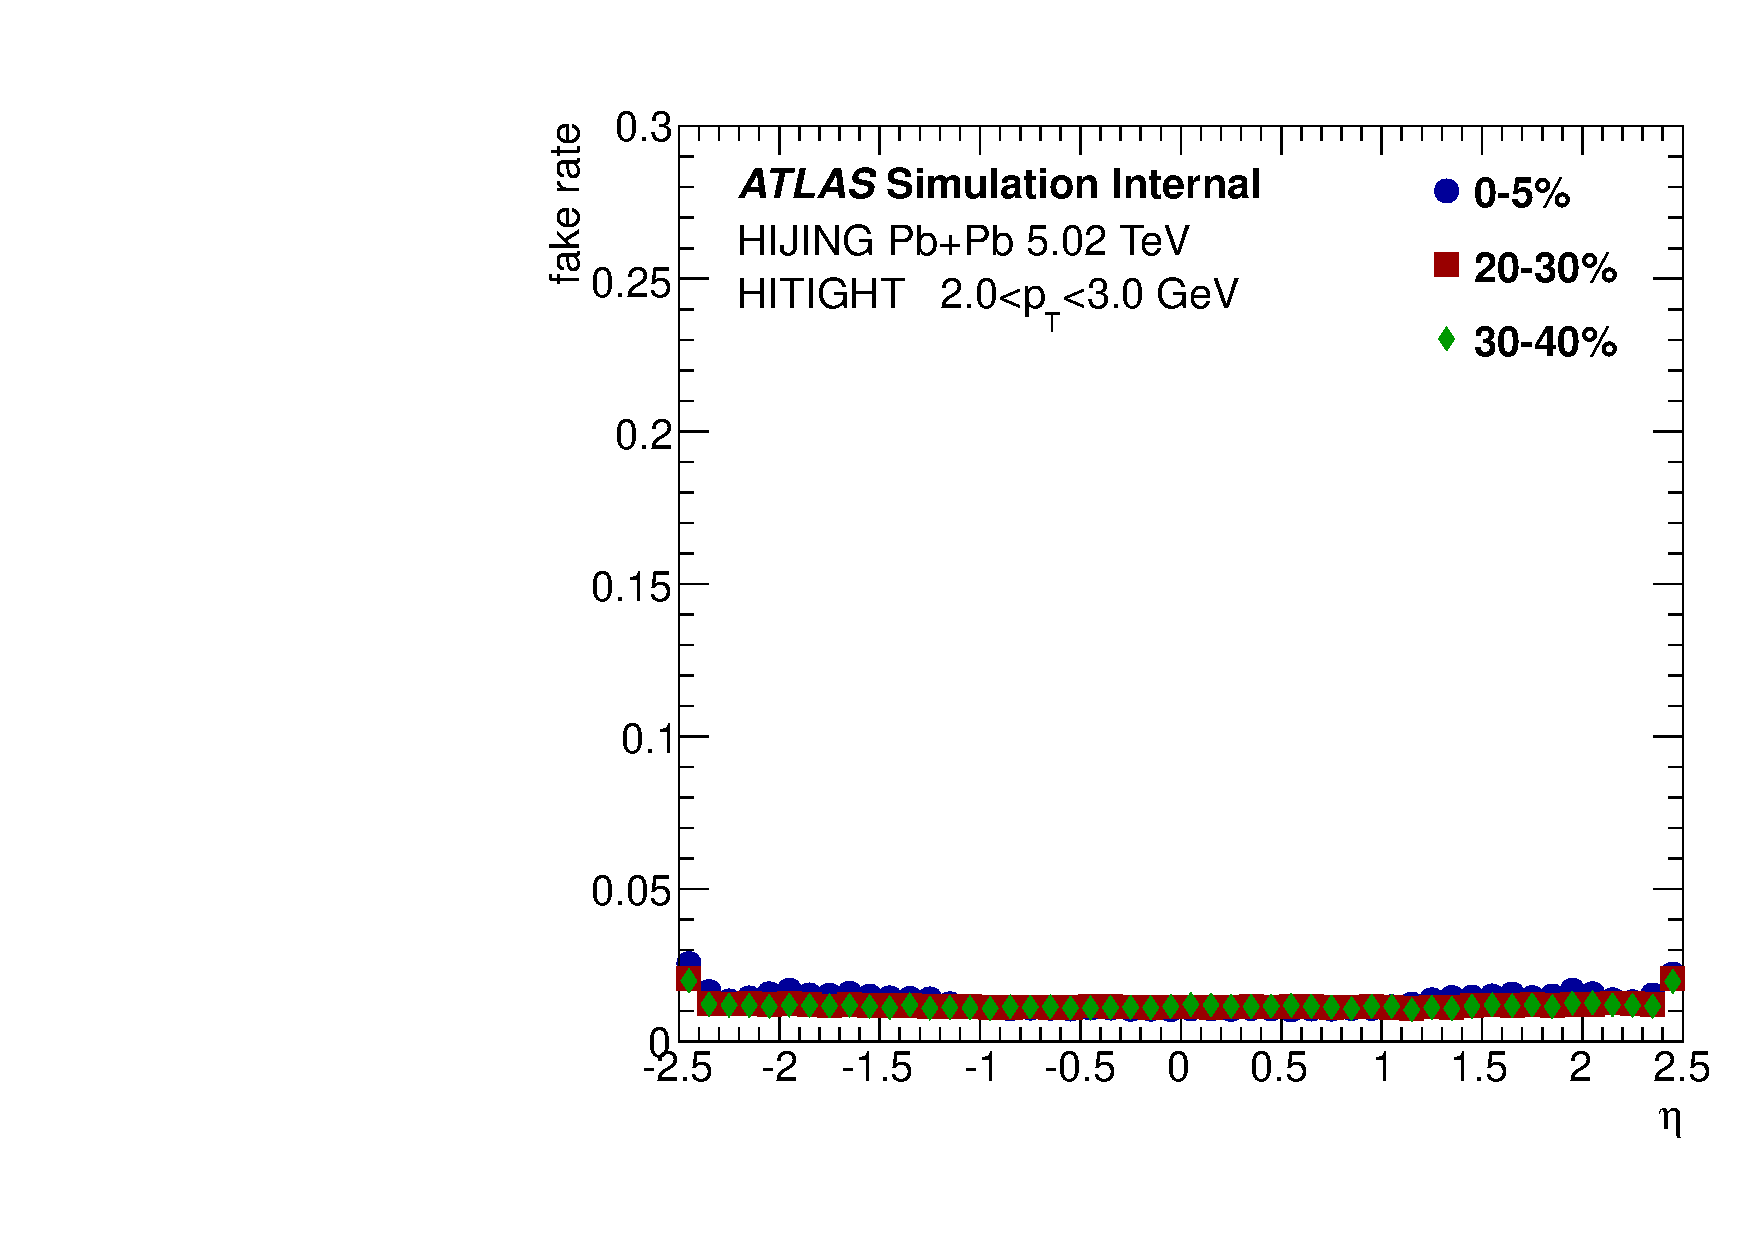
\includegraphics[width=.32\linewidth]{figs/sec_trkSel/PbPb502/PbPb502_TIGHT_fak_Pt4.pdf}
\caption{5.02 TeV Pb+Pb tracking fake rates $f(\eta)$, for different $p_{\text{T}}$ ranges and centralities. Top row is for loose track quality cut (default) and bottom row is for tight cut.}
\label{fig:PbPb502_trkFak}
\end{figure}



